I denne test køres programmet med de valgte værdier på symbolske konstanter, som ses på figur~\ref{fig:def} og indholdet i datafilen som ses figur~\ref{fig:info}.

\begin{figure}[!h]
  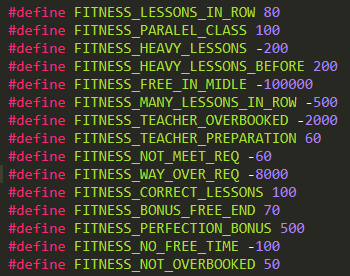
\includegraphics[scale = 1]{partials/graphics/programtestdef.png}
  \caption{Eksempel på programmets værdier af symbolske konstanter.}
  \label{fig:def}
\end{figure}

\begin{figure}[!h]
  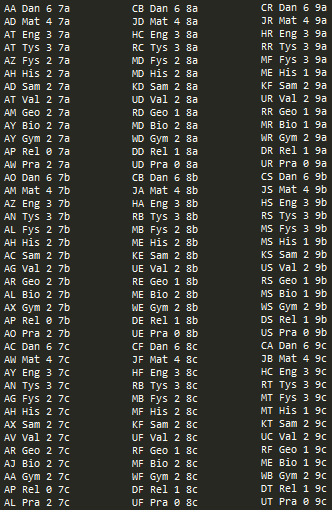
\includegraphics[scale = 1]{partials/graphics/programtestinfo.png}
  \caption{Eksempel på datafil.}
  \label{fig:info}
\end{figure}

På figur~\ref{fig:test} ses den valgte kombination af skemaer for det niende klassetrin, samt antallet af lektioner, der er kravet for hvert fag, ''Must have'', hvor mange gange, de har hvert fag, ''Have'', skemaets fitnessniveau og hvor mange fag skemaet har nok af ''perfectiongrade''. På sidste linje, ses det hvor mange gange skemaet har fag på samme tid som en parallelklasse, ''lessons with parallel'', og med begge parallelklasser, ''lessons with both''. Hvor mange gange, der er tunge fag efter, ''Heavy lessons after'', og før middag, og sidst hvor mange gange skemaet har lektioner, hvor læreren er lektioner i andre klasser.

\begin{figure}[!h]
  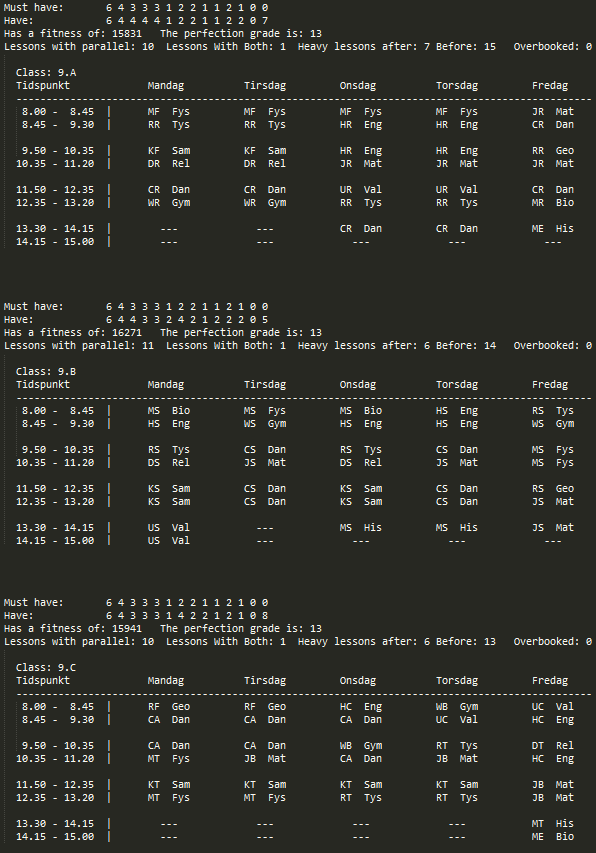
\includegraphics[scale = 1]{partials/graphics/programtestres.png}
  \caption{}
  \label{fig:test}
\end{figure}